\section{Трекинг на основе особых точек и цвета}\label{tracking}

Данный раздел содержит описание предлагаемого алгоритма трекинга,
комбинирующего в себе два подхода: основанный на ключевых точках
и основанный на цветах.
Сначала идет описание части метода, использующей точечные особенности
изображения.
Оно является достаточно кратким, поскольку рассказывает о довольно
распространенном и известном подходе.
Затем идет описание части, использующей цветовую информацию.
Оно является более подробным, поскольку касается менее общеизвестного
подхода и содержит некоторые модификации.
Завершается раздел описанием способа комбинирования цветового и точечного
алгоритмов.

\subsection{Трекинг на основе точечных особенностей изображения}
\label{subs:feat_tracking}

Применяемый в данной работе алгоритм трекинга с помощью точечных особенностей
представляет собой разновидность стандартного подхода "--- трекера
Канаде "--- Лукаса "--- Томаси
(KLT-трекера)\cite{LucasAndKanade,TomasiAndKanade,ShiAndTomasi,PyrLK}.
На кадрах с известной позицией объекта выделяются ключевые 2D-точки (точечные
особенности) и определяются соответствующие им 3D-точки на поверхности модели.
Движение ключевых точек от кадра к кадру отслеживается с помощью вычисления
оптического потока.
На кадре, для которого выполняется оценка позиции, по известным 2D-3D
соответствиям вычисляется положение объекта путем решения задачи
\PnP\cite{LepetitSurvey} с использованием RANSAC\cite{RANSAC} для отсеивания
выбросов.

\Comment{TODO: о порядке репроецирования 3D-точек, отбрасывании треков
и пересчете 3D-позиций рассказать подробнее в разделе про комбинирование.
Возможно, здесь нужно будет кратко на это сослаться.}

\subsection{Метод на основе распределения цвета}

\Comment{Во всем разделе плохо с обозначениями и формулами.}

\newcommand{\Hf}{\ensuremath{H_f}}
\newcommand{\Hb}{\ensuremath{H_b}}
\newcommand{\uvec}{\ensuremath{\vect{u}}}
\newcommand{\hedist}{\ensuremath{\HeX{\CDistX{\uvec}}}}
\newcommand{\HistLocal}{\ensuremath{H_i}}
\newcommand{\HistLocalFg}{\ensuremath{{\Hf}_i}}
\newcommand{\HistLocalBg}{\ensuremath{{\Hb}_i}}

Метод, использующий распределение цветов, направлен на нахождение такой
позиции, при которой контур наилучшим образом отделяет передний план от фона.
Это означает, что цвета на $\FgProj$ будет соответствовать цветам,
встречавшимся на переднем плане ранее в ходе трекинга, и наоборот: точки,
оказавшиеся на $\BgProj$, будут иметь цвет, характерный для фона.

Для учёта цветовой статистики строятся цветовые гистограммы, в которые
собираются данные о цветах точек в окрестности контура.
На кадре, где позиция объекта известна, окрестность контура $\CtLocal$
разбивается на несколько
непересекающихся областей~$\{\CtLocal_i\}_{i = 1}^n$.
Каждая из этих областей включает в себя часть переднего плана и часть фона:

\begin{equation}
\label{eqn:histo_partitioning}
\begin{array}{c}
\CtLocal_i = {\CtLocalFg}_i \cup {\CtLocalBg}_i \\
{\CtLocalFg}_i = \CtLocal_i \cap \CtLocalFg \\
{\CtLocalBg}_i = \CtLocal_i \cap \CtLocalBg
\text{.}
\end{array}
\end{equation}

Подробнее о том, как окрестность контура разбивается на локальные области,
будет
рассказано в следующем разделе.

На каждой из областей ${\CtLocalFg}_i, {\CtLocalBg}_i$ строится
гистограмма распределения цветов.
Гистограммы строятся таким образом, чтобы значения в каждом канале разбивались
на 32 ячейки, поэтому в этой главе под цветом пикселя $y$ будем понимать
множество цветов, попадающих в одну ячейку гистограммы:
$y \in \{0, 1, \dots, 31\}^3$.
В каждую ячейку гистограммы ${\HistLocal}_j$ записывается доля пикселей
соответствующих
цветов на её области ${\CtLocal_i}_j$.

Для данного цвета $y$ значения в гистограммах $\HistLocalFg(y)$ и
$\HistLocalBg(y)$ "--- это вероятности точки иметь цвет $y$, находясь
соответственно на переднем плане и на фоне.
Из-за того, что в каждой локальной области своя пара гистограмм, эти
вероятности могут быть разными на разных участках изображения.

\begin{align}
\label{eqn:H_f_Y}
    \HistLocalFg(y) &= \probX{I(\uvec) = y \mid \uvec \in \FgProj} \\
    \HistLocalBg(y) &= \probX{I(\uvec) = y \mid \uvec \in \BgProj}
\text{.}
\end{align}

Процесс получения позиции на новом кадре основан на максимизации апостериорной
вероятности позиции при данном изображении и данном наборе гистограмм.
Пусть дан новый кадр и некоторая позиция $\Pose$.
Спроецируем объект на изображение с использованием этой позиции.
Получим контур $\Contour$ и разбиение его окрестности на локальные области.
Тогда, как и в~\cite{Hexner2016}, вероятность того, что $\Pose$ является
позицией
объекта, можем оценить как

\begin{equation}
\label{eqn:pos_prob}
    \probMainX{\Pose} = \prod\limits_{\uvec \in \CtLocal} \left(
        \probF{\uvec} \hedist
        + \probB{\uvec} \left( 1 - \hedist \right)
    \right)
\text{.}
\end{equation}

Здесь $\He$ "--- приближение функции Хевисайда:

\begin{equation}
\label{eqn:heaviside}
    \HeX{x} = \frac{1}{\pi} \left( \arctan(\alpha x) - \frac{\pi}{2} \right)
\text{.}
\end{equation}

$\He$ оценивает вероятность того, что $\uvec$ лежит на переднем плане, с точки
зрения позиции объекта.
$\probF{\uvec}$ и $\probB{\uvec}$ "--- вероятности попадания на передний план и
на фон в соответствии с цветом точки:

\begin{align}
\label{eqn:Pfu}
    \probF{\uvec} &= \frac{\HistLocalFg(y)\eta_f}{\HistLocalFg(y)\eta_f +
        \HistLocalBg(y)\eta_b} \text{,} \\
    \probB{\uvec} &=\frac{\HistLocalBg(y)\eta_b}{\HistLocalFg(y)\eta_f +
        \HistLocalBg(y)\eta_b} \text{,}
\end{align}

где
$
    \eta_f = \sum\limits_{\uvec \in \CtLocal_i}\hedist
$ "--- количество точек переднего плана на $\CtLocal_i$,

$
    \eta_b = \sum\limits_{\uvec \in \CtLocal_i}(1 - \hedist)
$ "--- количество точек фона.


Таким образом, вероятность позиции $\Pose$ будет высокой, если точки области
$\CtLocalFg$ будут и по цвету классифицироваться как точки переднего плана, а
точки области $\CtLocalBg$ "--- как фон.

Функция энергии цветового трекинга получается логарифмированием и взятием с
минусом
формулы~\ref{eqn:pos_prob}:

\begin{equation}
\label{eqn:err_func}
\Energy(\xi) = - \sum\limits_{\uvec \in \CtLocal}
\log(\hedist \probF{\uvec} + (1 - \hedist)\probB{\uvec})
\text{.}
\end{equation}

Позиция объекта получается минимизацией функции энергии~\ref{eqn:err_func}.
Оптимизация проводится квазиньютоновским методом последовательного
квадратичного
программирования(SLSQP)~\cite{SLSQP}, аппроксимирующим гессиан функции.
Градиент вычисляется аналитически.
Вывод формулы градиента можно найти в~\cite{Tjaden2018}.
\Comment{Подсчет градиента разве не отличается от \cite{Tjaden2018}?}

Поскольку функция~\ref{eqn:err_func} может быть зашумлённой в неблагоприятных
для трекинга условиях, результат оптимизации может оказаться далеким от
истинной позиции.
Поэтому оптимизация проводится в ограниченной области с центром в точке
инициализации.
Для параметров переноса её ширина составляет $kd$, где $d$ "--- диаметр
объекта.
Ширина области для параметров поворота "--- $m$ радиан (в нашей реализации $d =
0.4, m = 1$).
При импорте модели она масштабируется так, чтобы её диаметр равнялся $5$,
чтобы масштаб объекта не влиял на соотношение между осями поворота и переноса.

\Comment{Про оптимизацию на пирамиде не сказано. В реализации пирамида сейчас
тоже не используется}

После получения новой позиции на каждом следующем кадре строятся новые
гистограммы, которые взвешенно суммируются со старыми: 

\begin{align}
\HistLocalFg &= \alpha_f \HistLocalFg^{\text{\it new}} + (1 - \alpha_f)
\HistLocalFg^{\text{\it old}} \\\HistLocalBg &= \alpha_b
\HistLocalBg^{\text{\it new}} + (1 - \alpha_b) \HistLocalBg^{\text{\it
old}}\text{,}
\end{align}

где $\alpha_f, \alpha_b$ - коэффициенты обновления (в нашей реализации
$\alpha_f = 0.1, \alpha_b = 0.2$).

\Comment{Про цветовые пространства здесь не говорится. Это уже обработка
входных изображений, и она даёт значимое преимущество только на отдельном
цветовом методе.
На комбинированном общий результат слабо отличается }

\subsubsection*{Разбиение на локальные области}

В нашей реализации окрестность контура разбивается на $32$ локальные области,
для
каждой из
которых поддерживается одна пара гистограмм.

Для каждой точки $\uvec \in \CtLocal_i$ при вычислении $\probF{\uvec}$ и
$\probB{\uvec}$ по
формулам~\ref{eqn:Pfu} выбирается соответствующая пара $\left( \HistLocalFg,
\HistLocalBg \right)$.

Оптимизация функции ошибки~\ref{eqn:err_func} направлена на нахождение такой
позиции, при которой контур лучше всего отделяет передний план от фона, поэтому
её вычисление проводится по полосе вокруг контура ширины $2r$ (в нашей
реализации $r = 40$).
Таким образом, требуется разбить на области эту полосу.
Области должны, по возможности, содержать примерно равное количество точек
переднего плана и фона, то есть внутренней и внешней частей полосы.
Поэтому они строятся так, чтобы контур проходил по середине
области.
Область точки на полосе совпадает в нашем решении с областью ближайшей к ней
точки на контуре (рис.~\ref{fig:fb_contour}).

\begin{figure}[t]
\centering
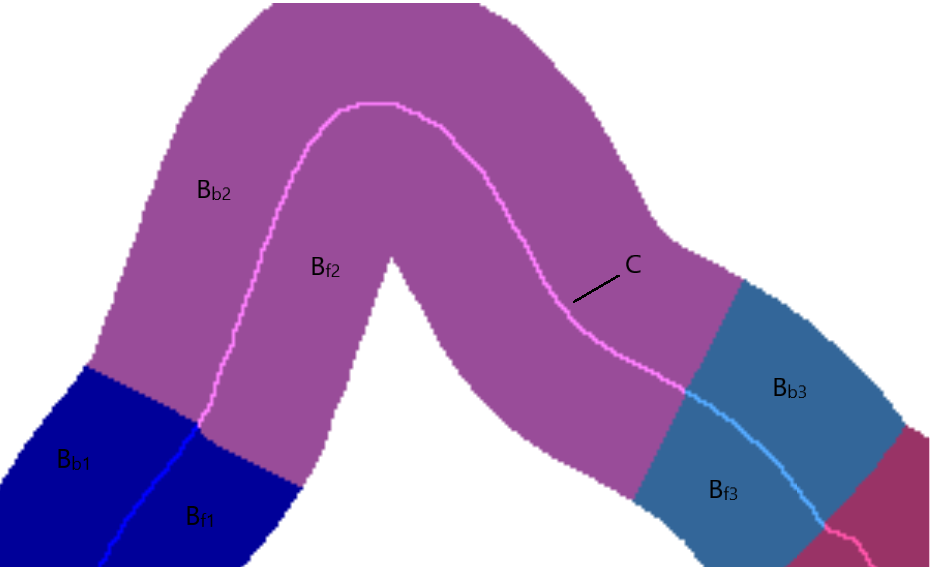
\includegraphics[width=\textwidth]{fig/fb_contour.png}
\caption{
Разбиение на области ${B_f}_i, {B_b}_i$ полосы вокруг контура, по которой
вычисляется функция ошибки
} \label{fig:fb_contour}
\end{figure}

Таким образом, достаточно разбить на области точки контура.
Для этого мы разбиваем на несколько участков поверхность трёхмерной модели
объекта: объект помещается в центр единичной сферы, а сама сфера разбивается
на $32$ равные по площади части по зенитным и азимутным углам.
Каждую точку объекта можно отнормировать, чтобы она попала на поверхность
сферы, и таким образом поделить на области поверхность объекта
(рис.~\ref{fig:color-object-areas}).
Проекция объекта позволяет поделить на области контур
(рис.~\ref{fig:projected-areas}).

\begin{figure}[t]
\centering
\begin{minipage}[h]{0.49\linewidth}
\center{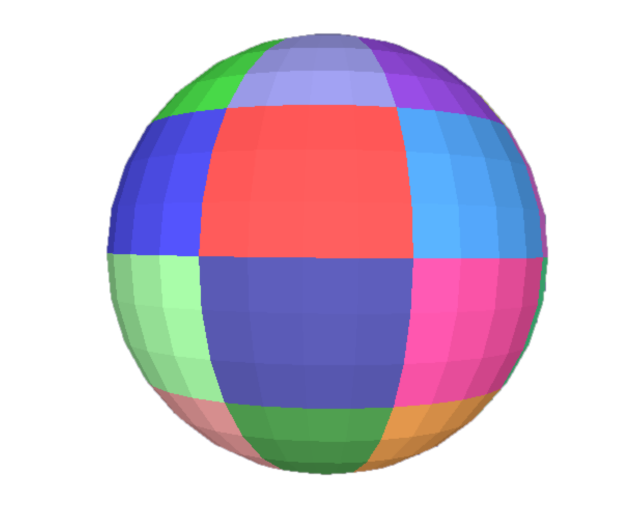
\includegraphics[width=0.8\linewidth]{fig/sphere_straight.png}}
\end{minipage}
\hfill
\begin{minipage}[h]{0.49\linewidth}
\center{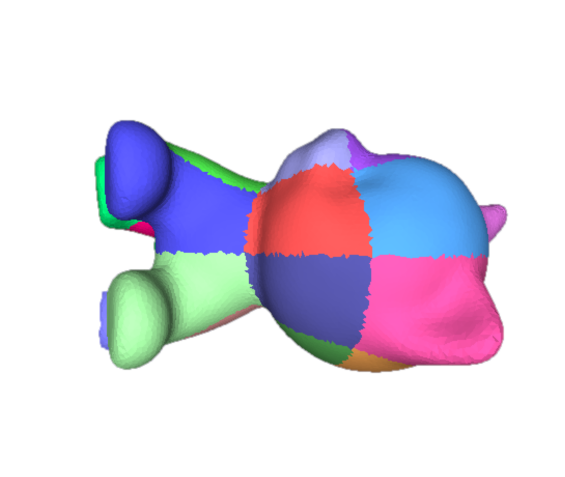
\includegraphics[width=0.8\linewidth]{fig/cat_straight.png}}
\end{minipage}
\caption{Разбиение на локальные области поверхностей сферы и объекта}
\label{fig:color-object-areas}
\end{figure}

\begin{figure}[t]
\centering
\begin{minipage}[h]{0.49\linewidth}
\center{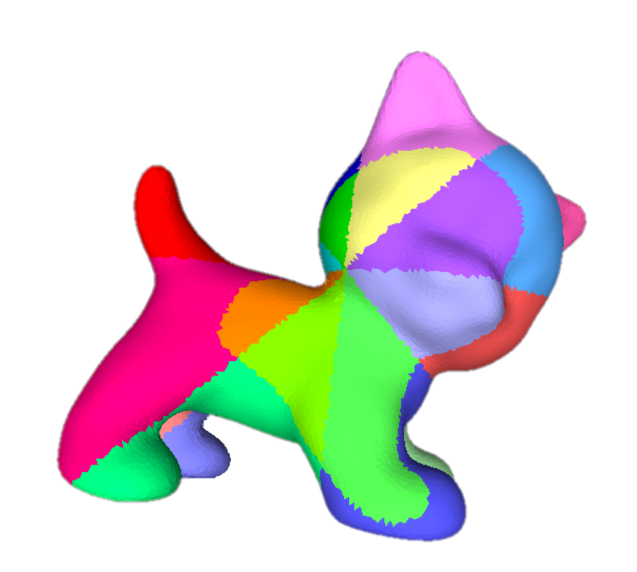
\includegraphics[width=0.8\linewidth]{fig/cat_transformed.png}}
\end{minipage}
\hfill
\begin{minipage}[h]{0.49\linewidth}
\center{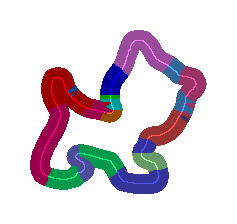
\includegraphics[width=0.8\linewidth]{fig/cat_contour.png}}
\end{minipage}
\caption{Слева разбиение на области 3D-модели объекта. Проекция объекта
разбивает на области контур (правое изображение). Точки вокруг контура
поппадают в ту же область, что и ближайшие точки на контуре. }
\label{fig:projected-areas}
\end{figure}

Такое разделение объекта неизменно между кадрами, поэтому цветовую информацию
в гистограммах можно накапливать в ходе трекинга.
Данные в гистограммах $\HistLocalFg$ будут при этом отражать распределение
цветов на определённых областях объекта, а данные в гистограммах $\HistLocalBg$"--- распределение цветов на фоне вокруг этих областей.
Количество гистограмм при этом относительно небольшое и можно 
обновлять их все на каждом кадре.

На локальные области разделяется объект целиком. 
Очевидно, что на отдельном кадре только часть областей будут спроецированы на
контур и поучаствуют в разбиении изображения.
Поэтому информация в некоторых гистограммах может не набираться на протяжении
большого количества кадров.
После поворота объекта такие области могут нам понадобиться, но информации в
их гистограммах будет недостаточно.
Для решения этой проблемы ведётся учёт <<опыта>> локальных гистограмм и
заводится одна глобальная гистограмма.

Если опыт $s_{\text{\it local}}$ пары гистограмм $\left( \HistLocalFg,
\HistLocalBg \right)$меньше некоторого порога
$s_{\text{\it suff}}$, то для точек области $\ImgDom_i$ $\Hf(y)$ и $\Hb(y)$
вычисляются
как
взвешенные суммы локальных и глобальных гистограмм:

\begin{align}
\label{eqn:histo_skill}
\Hf(y) &= \dfrac{s_{\text{\it local}} \HistLocalFg + (s_{\text{\it suff}} -
s_{\text{\it local}})
        {H_{\text {\it global}}}_f}{s_{\text{\it suff}}} \\
\Hb(y) &= \dfrac{s_{\text{\it local}} \HistLocalBg + (s_{\text{\it suff}} -
s_{\text{\it local}})
        {H_{\text {\it global}}}_b}{s_{\text{\it suff}}}
\text{.}
\end{align}

Порог $s_{\text{\it suff}}$ выбирается как среднее значение опыта по всем
локальным
гистограммам.
Опыт локальной гистограммы оценивается как общее количество пикселей, попавших
когда-либо в её область.
Чтобы значение опыта соответствовало уровню знаний о последних кадрах, на
каждом кадре его значение домножается на коэффициент, меньший единицы:

\begin{equation}
s_{\text{\it local}} = \alpha_f s_{\text{\it local}}^{\text{\it new}} + (1 -
\alpha_f) s_{\text{\it local}}^{\text{\it old}}
\text{.}
\end{equation}

\Comment{TODO: описать то, как выбираются гистограммы.}

\subsection{Комбинирование методов}

\Comment{В чем суть комбинирования, просто поиск исходной позиции ключевыми
точками? Не только: еще и правильное согласование новой позиции и ключевых
точек. Оно заключает в себе: (1) репроецирование новых точек уже из новой
позиции, пересчет старых точек и отбрасывание точек с невидимых граней можно
тоже сюда же записать.}

Первый способ скрещивания алгоритмов заключается в последовательном их
применении и инициализации одного метода другим.
Вычисление цветовой функции ошибки~\ref{eqn:err_func} вместе с определением
локальной области для каждой точки и вычисление градиента занимают достаточно
много времени.
Поэтому для скорости трекинга важно сократить количество итераций, за которое
сходится оптимизация функции.
Этого можно достичь хорошей её инициализацией, близкой к глобальному
минимуму.
В этом методе роль такой оптимизации играет алгоритм ключевых точек.

\newcommand{\FeatAlg}{\ensuremath{F_{\text{\it feat}}}}
\newcommand{\ColorAlg}{\ensuremath{F_{\text {\it color}}}}
\newcommand{\PoseOnFrame}[1]{\ensuremath{\Pose^{\left( #1 \right)}}}
\newcommand{\PoseI}{\ensuremath{\PoseOnFrame{i}}}
\newcommand{\FeatPoseI}{\ensuremath{\PoseI_{\text {\it feat}}}}
\newcommand{\FeatPose}{\ensuremath{\Pose_{\text {\it feat}}}}

\newcommand{\XOld}{\ensuremath{\homv{x_{\text {\it old}}}}}
\newcommand{\XNew}{\ensuremath{\homv{x_{\text{\it new}}}}}
\newcommand{\ReprErr}[1]{\ensuremath{\homv{e}( #1 )}}

Позиции объекта на видео определяются последовательно, от кадра к кадру.
Введём обозначения:

\begin{enumerate}
\item $\FeatAlg(\Img)$ "--- результат работы алгоритма ключевых точек на
изображении $\Img$;
\item $\ColorAlg(\Pose, \Img)$ "--- результат работы цветового алгоритма на
изображении $\Img$
при инициализации его позицией $\Pose$.
\end{enumerate}

Тогда при обработке $i$-ого кадра проводится следующая последовательность
действий:

\begin{enumerate}
\item Чтение изображения $\Img_i$
\item Вычиление позиции алгоритмом ключевых точек:
    $\FeatPoseI = \FeatAlg(\Img_i)$
\item Уточнение позиции цветовым методом:
    $\PoseI = \ColorAlg(\FeatPoseI, \Img_i)$
\item Вычисление  3D-позиций, соответствующих ключевым особенностям, с
    использованием позиции $\PoseI$
\item $\PoseI$ сохраняется в качестве итоговой позиции
\end{enumerate}

После получения изображения проиходит вычисление позиции $\FeatPoseI$
алгоритмом
ключевых точек, описанным в главе~\ref{subs:feat_tracking}.
Чаще всего эта позиция близка к глобальному минимуму функции энергии цветового
алгоритма, но если метод ключевых точек отработал плохо (например из-за
смазанности изображения), то эта позиция может оказаться далеко от оптимума, и
из-за этого цветовой алгоритм может не сойтись.
Чтобы избежать таких случаев, предусмотрен альтернативный способ инициализации
цветового метода.

Наиболее естественный способ инициализировать алгоритм трекинга при отсутствии
специального метода инициализации "--- это взять позицию с предыдущего кадра.
Но очень часто неправильная работа трекинга на ключевых точках вызвана
смазанностью при быстром движении объекта.
Чтобы учесть это движение, мы вычисляем альтернативную позицию экстраполяцией
движения с предыдущих кадров:

\begin{equation}
\label{eqn:extrapolation}
\PoseI_{\text{\it ex}} = \Delta \Pose \PoseOnFrame{i - 1} = \PoseOnFrame{i -
1}(\PoseOnFrame{i - 2})^{-1} \PoseOnFrame{i - 1}
\text{.}
\end{equation}

Эта позиция выбирается, если функция энергии цветового алгоритма на ней будет
меньше.

\begin{equation}
\label{eqn:init_selection}
\Pose_{\text{\it color init}} = \argmin(\Energy(\FeatPose),
\Energy(\Pose_{\text{\it ex}}))
\end{equation}

Позиция $\PoseI$, полученная цветовым методом, считается уточнённой
посравнению с позицией $\FeatPoseI$.
Поэтому она может быть использована, чтобы скорректировать метод ключевых
точек.

Позиция $\PoseI$ используется для того, чтобы получить 3D-прообразы
ключевых точек, обнаруженных впервые.
При этом запоминается тот полигон, на котором лежит прообраз.
Кроме того, для точек, наблюдавшихся на предыдущих кадрах, 3D-позиция также
пересчитывается заново с использованием $\PoseI$.
Она будет использоваться в дальнейшем вместо старой 3D-позиции в случае, если
окажется точнее неё.

Точность 3D-позиции определяется ошибками её репроекции на всех кадрах, где
отслеживалась соответствующая ключевая точка.
Пусть $\XOld$ "--- старая 3D-позиция, а $\XNew$ "--- новая. 
Пусть также ключевая точка была сдетектирована на изображениях начиная с
$\Img_k$
до текущего кадра $\Img_l$, и её 2D-позициями на этих кадрах были $\uvec_k ...
\uvec_l$
соответственно.
Тогда суммарной ошибкой репроекции 3D-точки $x$ будет

\begin{equation}
\label{eqn:sum_reproj}
\ReprErr{\homv{x}} = \sum\limits_{i = k}^l \| \homv{\uvec_i} - \CamIntr \cdot
[\RotMat_i \mid \TrVec_i] \cdot \homv{x} \|
\end{equation}

Старая позиция заменяется на новую, если $\ReprErr{\XNew} < \ReprErr{\XOld}$.
Так цветовой трекинг позволяет уточнить 3D-прообразы ключевых точек, тем самым
делая трекинг на ключевых точках более устойчивым.

Кроме того, с помощью уточнённой позиции проводится фильтрация выбросов:
исключаются из рассмотрения те 2D-3D-соответствия, для которых ошибка
репроекции из уточнённой позиции больше определённого порога.
Также удаляются точки, которые не попадают на передний план, то есть не лежат
на проекции объекта.
Если некоторый полигон не виден на переднем плане, то точки, лежащие на нём,
считаются невидимыми и тоже далее не рассматриваются.
Таким образом, уточнение позиции цветовым трекингом позволяет отфильтровать
часть 2D-3D соответствий, не согласующихся с позицией.

\Comment{Дальше идёт описание старого метода обновления 3D-позиций. В итоге
будет оставлен один из них}

Чтобы определить, какая позиция лучше, нужно оценить ошибку репроекции для
каждой позиции.
Но ошибка репроекции будет нулевой для кадра, по которому позиция вычислена,
поэтому нужно выбрать какой-то кадр, на котором обе ошибки будут отличны от
нуля.
Вопрос об обновлении позиции откладывается до следующего кадра, и решается уже
по репроекции на нём.

Пусть $\uvec_{i + 1}$ "--- позиция точечной особенности на кадре $\Img_{i +
1}$.
Пусть $\XOld$ "--- её старая 3D-позиция, а $\XNew$ "--- новая. 

Тогда ошибкой репроекции на кадре $\Img_{i + 1}$ будет

\begin{equation}
\label{eqn:err_reproj}
\ReprErr{\homv{x}} = \| \homv{\uvec_{i + 1}} - \CamIntr \cdot
[\RotMat_{i + 1} \mid \TrVec_{i + 1}] \cdot \homv{x} \|
\end{equation}

Старая позиция заменяется на новую, если $\ReprErr{\XNew} < \ReprErr{\XOld}$.
